% !Mode:: "TeX:UTF-8"


%-------------------------------------------------------------------------------
% This file provides a skeleton ATLAS document.
%-------------------------------------------------------------------------------
% \pdfoutput=1
% The \pdfoutput command is needed by arXiv/JHEP/JINST to ensure use of pdflatex.
% It should be included in the first 5 lines of the file.
%-------------------------------------------------------------------------------
% Specify where ATLAS LaTeX style files can be found.


%maybe uncomment:\newcommand*{\ATLASLATEXPATH}{latex/}

% Use this variant if the files are in a central location, e.g. $HOME/texmf.
% \newcommand*{\ATLASLATEXPATH}{}


% \newcommand{\stopFootnote}{%
% The superpartners of the left- and right- handed
%   top quarks, $\stopL$ and $\stopR$,
%   mix to form the two mass eigenstates $\stopone$ and $\stoptwo$, where
%   $\stopone$ is the lighter one. Throughout this note $\stopone$ is
%   noted as $\stop$.}

%\newcommand{\AtlasCoordFootnote}{%
%ATLAS uses a right-handed coordinate system with its origin at the nominal interaction point (IP)
%in the centre of the detector and the $z$-axis along the beam pipe.
%The $x$-axis points from the IP to the centre of the LHC ring,
%and the $y$-axis points upwards.
%Cylindrical coordinates $(r,\phi)$ are used in the transverse plane, 
%$\phi$ being the azimuthal angle around the $z$-axis.
%The pseudorapidity is defined in terms of the polar angle $\theta$ as $\eta = -\ln \tan(\theta/2)$.
%Angular distance is measured in units of $\Delta R \equiv
%\sqrt{(\Delta\eta)^{2} + (\Delta\phi)^{2}}$. The transverse momentum
%is the momentum component in the transverse plane.}


%-------------------------------------------------------------------------------
%\documentclass[UKenglish,texlive=2013,PAPER,coverpage]{\ATLASLATEXPATH atlasdoc}
\documentclass[
dissertation,
copyright,
final,
justified,
numbers,
sort&compress,
numsections,
gsmodern,
]{uothesis}

% The language of the document must be set: usually UKenglish or USenglish.
% british and american also work!
% Commonly used options:
%  texlive=YYYY          Specify TeX Live version (2013 is default).
%  atlasstyle=true|false Use ATLAS style for document (default).
%  coverpage             Create ATLAS draft cover page for collaboration circulation.
%                        See atlas-draft-cover.tex for a list of variables that should be defined.
%  cernpreprint          Create front page for a CERN preprint.
%                        See atlas-preprint-cover.tex for a list of variables that should be defined.
%  PAPER                 The document is an ATLAS paper (draft).
%  CONF                  The document is a CONF note (draft).
%  PUB                   The document is a PUB note (draft).
%  txfonts=true|false    Use txfonts rather than the default newtx - needed for arXiv submission.
%  paper=a4|letter       Set paper size to A4 (default) or letter.

%-------------------------------------------------------------------------------
% Extra packages:
%\usepackage{\ATLASLATEXPATH atlaspackage}
% Commonly used options:
%  biblatex=true|false   Use biblatex (default) or bibtex for the bibliography.
%  backend=biber         Use the biber backend rather than bibtex.
%  subfigure|subfig|subcaption  to use one of these packages for figures in figures.
%  minimal               Minimal set of packages.
%  default               Standard set of packages.
%  full                  Full set of packages.
%-------------------------------------------------------------------------------
% Style file with biblatex options for ATLAS documents.
%\usepackage{\ATLASLATEXPATH atlasbiblatex}

% Package for creating list of authors and contributors to the analysis.
%\usepackage{\ATLASLATEXPATH atlascontribute}

% Useful macros
%\usepackage{\ATLASLATEXPATH atlasphysics}

% See doc/atlas-physics.pdf for a list of the defined symbols.
% Default options are:
%   true:  journal, misc, particle, unit, xref
%   false: BSM, hion, math, process, other, texmf
% See the package for details on the options.
\usepackage{graphicx}

\usepackage{atlasphysics}

\usepackage{float}
%\usepackage{floatrow}
%\floatsetup[table]{capposition=top}
\usepackage{tabularx}
\usepackage{pdflscape}
\usepackage{siunitx}
\usepackage{footnote}
\usepackage{footnotebackref}
\usepackage{tocbibind}
\usepackage{enumitem}

\usepackage{epsfig}
\usepackage{epstopdf}
%\usepackage{subcaption}
%\usepackage{caption}

\usepackage{enumerate}
\usepackage{rotating} %GR added
%\usepackage{mdwlist}
\usepackage{multirow}
\usepackage{multicol}
\usepackage{pdflscape}
\usepackage{longtable}
\usepackage{slashed}
\usepackage{verbatim}
\usepackage{hyperref} %If you get an error due to hyperref package, delete your old INT.aux file then recompile.
\usepackage{tikz}
\usepackage[compat=1.1.0]{tikz-feynman}
%\usepackage{multirow}
\usepackage{slashed}
\usepackage{smartdiagram}

\usepackage{booktabs} %Use for smarter Tables
\usepackage{pifont}
\usepackage{tabu}
\usepackage{amsmath}
\usepackage{slashed}
\usepackage{color}
\usepackage{placeins}
\usepackage{xspace}
\usepackage{adjustbox}
\usepackage{dcolumn}
\usepackage[flushleft]{threeparttable}

\usepackage[style=numeric-comp,backend=biber,sorting=none]{biblatex}
%\usepackage[hang,center]{subfigure}
%\usepackage{subfigure}

%\captionsetup[figure]{labelformat=parens, labelsep=newline}

% set up labelformat and labelsep for subfigure

\captionsetup[subfigure]{labelformat=simple}%, labelsep=period}%, labelsep=colon}
 


%\usepackage[utf8]{inputenc}

% Files with references for use with biblatex.
% Note that biber gives an error if it finds empty bib files.

\addbibresource{thesis.bib}

%\addbibresource{bibtex/bib/ATLAS.bib}
%\bibliography{thesis.bib}
%% Paths for figures - do not forget the / at the end of the directory name.
\graphicspath{{logos/}{figures/}}

% Add you own definitions here (file atlas-document-defs.sty).
%\usepackage{atlas-document-defs}

%-------------------------------------------------------------------------------
% Generic document information
%-------------------------------------------------------------------------------

%% Title, abstract and document 
%\input{atlas-document-metadata}

%% Author and title for the PDF file
\hypersetup{pdftitle={ATLAS document},pdfauthor={The ATLAS Collaboration}}

%-------------------------------------------------------------------------------
% Content
%-------------------------------------------------------------------------------
\newcommand{\Lagr}{\mathcal{L}}
%\setlength\parindent{0pt}


\usepackage{lineno, lipsum}
%\RequirePackage{lineno}
%\linenumbers


\begin{document}
%\begin{linenumbers}


\thispagestyle{empty}
\begin{center}
SEARCH FOR HIGGS BOSON PAIR PRODUCTION IN THE FULLY BOOSTED ${b\overline{b}WW\text{*}}$ CHANNEL IN ${\sqrt{s}}$ =  13 TeV PROTON-PROTON COLLISIONS AT THE LARGE HADRON COLLIDER USING THE ATLAS DETECTOR

\vspace*{\fill}
by\\
JOHN CHRISTOPHER STEPHEN MYERS
\vspace*{\fill}

A DISSERTATION \\
Presented to the Department of Physics and the Graduate Scool of the University of Oregon in partial fulfillment of the requirements for the degree of Doctor of Philosophy\\~\\
March 2019
\end{center}
%\abstract{
This dissertation presents a search for double Higgs production in the ${b\bar{b}WW^{*}}$ final state in proton-proton collisions at the ATLAS detector at the Large Hadron Collider. Double Higgs production is predicted in the Standard Model with a cross section of ${\sigma_{HH} = 33.53^{+4.3\%}_{-6.0\%}\pm{5.9\%}}$ fb. Many Beyond the Standard Model theories predict enhancements to the production cross section through resonant production. 
\indent The 2015-2016 ATLAS dataset has an integrated luminosity of 36.1 fb\textsuperscript{-1} with a center of mass energy of ${\sqrt{s} = 13 TeV}$. Candidate events are broken into two kinematic regions: a resolved selection containing one lepton (either an electron or muon), 2 b-tagged calorimeter jets, 2 light-flavor jets, and missing transverse energy; and a boosted analysis containing one lepton (electron or muon), two large radius jets, one with two ghost associated, b-tagged track-jets and missing transverse energy. No significant deviation from background was observed a cross section upper limit was set for the SM double Higgs production of 10 pb and for resonant production as a function of HH invariant mass from 500 GeV to 3000 GeV.
}
%\school{University of Oregon, Eugene, Oregon}%Graduate school
\school{The Ohio State University, Columbus, Ohio}%Undergraduate school

\degree{Doctor of Philosophy, Physics, 2018 University of Oregon}
\degree{Bachelor of Science, Physics, 2013, The Ohio State University}


%%There is a known issue if you do not fill in the interests section.  If you want to skip this section, comment out line#526 of uothesis.cls file \cvitem{GRANTS, AWARDS AND HONORS}{\@awards}
\interests{Boosted object reconstruction}
\interests{Trigger and detector operations}

\position{Graduate Research Assistant, University Of Oregon: ATLAS Collaboration, 2015-Present}%Your job while at UO, probably graduate research assistant.
\position{Graduate Teaching Assistant, University Of Oregon: Department of Physics, 2013-2015}

\award{}%If you didn't get any awards you'll have to comment out things in the uothesis. I dug up something from my undergraduate
\publication{List of publications with significant contributions:}
\publication{\fullcite{Aaboud2019}}
\publication{Co-authored on 124 publications with minor contributions can be found at Inspire (search parameters: exactauthor:John.Myers.1)}
%Fill this out with your publications.

%\input{acknowledgements}

%\maketitle



%\tableofcontents

%%%%Use this as a filler to get the template working

TESTING  \cite{ATL-PHYS-PUB-2015-015}
%\include{introduction}
%\include{motivations}
%\include{experiment}
%\include{gFEX}
%\include{analysisoverview}
%\include{combinedPerformance}
%\include{analysis}
%\include{conclusions}

%\begin{appendices}
\appendix
%\include{sanityChecks}
%\appendix
%\include{signalContamination}
%\end{appendices}
%\end{linenumbers}

%% List of contributors - print here or after the Bibliography.
%%\PrintAtlasContribute{0.30}
%%\clearpage
%
%%-------------------------------------------------------------------------------
%%%%%Use this as a filler to get the template working
%%Introduction
\chapter{Introduction}
The Standard Model (SM) is the culmination of more than a century of work. The first piece added to the puzzle was the electron, discovered in 1891. Since then, 24 other particles have been discovered, with the final piece, the Higgs Boson, being added in 2012. Since it was theorized, the SM has held up to rigorous experimentation and remains an unbeaten theory of fundamental matter and forces. Even though the SM is widely successful, it fails to explain all observed phenomena. Gravity, neutrino masses, dark matter, along with other observations, all lacking explanation within the SM. The remaining task is to probe the extremes of the SM to either more precisely measure the parameters or to find its limit.
%Include this is a search for BSM production
\section{The Standard Model}
The Standard Model defines the basic building blocks of matter and force and the interactions between them. Normal matter that we interact with on a daily basis is made of protons, neutrons, and electrons. Electrons are a fundamental particle, called a lepton, meaning they are not made of smaller constituents. However, protons and neutrons are not fundamental particles. They are a composite of up and down quarks, two more fundamental particles. The protons are made of 2 ups and a down and the neutrons are made of two downs and an up. Leptons and quarks are both different types of fermions. \linebreak
\indent Fermions are spin-${\frac{1}{2}}$ particles that make up all matter in the SM. The fermions can be broken down into 3 "generations". Where a generation contains two quarks, one with electric charge ${+\frac{2}{3}}$ and one with electric charge ${-\frac{1}{3}}$, one electrically charged lepton, charge -1, and one electrically neutral lepton. The quarks have an additional color charge, of which there are 3 charges. This is additional quantum number associated with the strong force. In all, this gives 12 fermions. \linebreak 

\begin{table}[h]
\begin{center}
\footnotesize
\begin{tabular}[h]{|c||c|c|c|c|}
\hline
 & Particle & Spin & Charge & Mass \\
\hline\hline
Quarks &&&&\\
\hline
u type &u& & &${2.4^{+0.6}_{-0.4} MeV}$\\
 &c&${\frac{1}{2}}$&${\frac{2}{3}}$&${1.28\pm{0.03} GeV}$\\
 &t& & &${173.1\pm{0.6} GeV}$\\
\hline
d type & d& & & ${4.7^{+0.5}_{-0.4} MeV}$\\
 & s & ${\frac{1}{2}}$ & ${-\frac{1}{3}}$ & ${96^{+8}_{-4} MeV}$\\
 & b & & & ${4.18^{+0.04}_{-0.03} GeV}$\\
\hline\hline
Leptons &&&&\\
\hline
e family & e & ${\frac{1}{2}}$ & -1 &${0.5109989461\pm{}0.000000003 MeV}$\\
 & ${\nu_{e}}$ & & 0 & ${< 2 eV}$\\
 \hline
${\mu}$ family & ${\mu}$ & ${\frac{1}{2}}$ & -1 &${105.6583745\pm{}0.0000024 MeV}$\\
 & ${\nu_{\mu}}$ & & 0 & ${< 2 eV}$\\
 \hline
${\tau}$ family & ${\tau}$ & ${\frac{1}{2}}$ & -1 &${1776.86\pm{}0.12 GeV}$\\
 & ${\nu_{\tau}}$ & & 0 & ${< 2 eV}$\\
 \hline\hline
 Bosons &&&&\\
 \hline
 Vector & ${\gamma}$ & 1 & 0 & ${< 10^{-18} eV}$\\
 & ${g}$ & 1 & 0 & ${0}$\\
 & ${W}$ & 1 & ${\pm}$ & ${80.385\pm{}0.0015 GeV}$\\
 & ${Z}$ & 1 & 0 & ${91.1876\pm{}0.0021 GeV}$\\
 \hline
 Scalar & H & 0& 0 & ${125.09\pm{}0.21\pm{}0.11 GeV}$\\
 \hline
\end{tabular}
\caption{Particles of the Standard Model (ref XXX (ian or PDG))}
\label{tab:SM}
\end{center}
\end{table}

\indent Gauge bosons are spin-${1}$ particles responsible for carrying the fundamental forces in the standard model. There are 12 physical gauge boson. The photon ${\gamma}$ is a massless, charge neutral force carrier for the electromagnetic force. The nuclear forces are carried by 3 massive gauge bosons. A chargeless Z boson and two charged W bosons, ${Q = \pm 1}$. Together, these 4 bosons control the electroweak interactions in the standard model. The remaining 8 bosons are the gluons, the force carriers for the strong nuclear interaction. Gluons are massless, electrically neutral particles that have two color charges. There is a gluon for each combination of the three color charges, giving the 8 total gluons. \linebreak
\indent The remaining piece of the standard is the Higgs Boson. The Higgs boson is a massive Scalar, spin-${0}$, chargeless boson. The Higgs boson is responsible for giving mass to the massive electoweak bosons through electroweak symmetry breaking. The particles and their properties are in Table ~\ref{tab:SM}\linebreak
\subsection{Interactions}
The SM is governed by three different types of interactions. For leptons, the overarching theory is quantum electrodynamics (QED). QED describes how particles behave under electroweak interactions. This can be broken down further into the electromagnetic interaction and the weak interaction. The electromagnetic interaction defines the interaction of electrically charged particles with photons. The fundamental diagram for the electromagnetic interaction is electron-positron annihilation ~\ref{Fey:e-p}. Where an electron and a positron collide and produce two photons. This can also be reversed, two photons interact and produce an electron-positron pair. The strength of this interaction is the electrical charge e. \linebreak

\begin{figure}[h]

\begin{center}
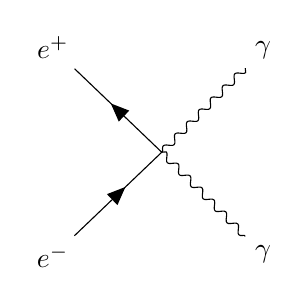
\begin{tikzpicture}
\begin{feynman}
\vertex (c) ;
\vertex [below left =of c] (i1){\(e^{-}\)};
\vertex [above left=of c] (i2) {\(e^{+}\)};
\vertex [below right=of c] (f1){\(\gamma\)};
\vertex [above right= of c] (f2){\(\gamma\)};
\diagram* {
(i1) -- [fermion] (c) -- [fermion] (i2) ,
(f1) -- [photon] (c)-- [photon] (f2)
};
\end{feynman}
\end{tikzpicture}
\caption{Electron-Positron Annihilation}
\label{Fey:e-p}
\end{center}
\end{figure}

\indent The weak interaction defines the interaction of particles under the weak isospin quantum number. There are two copies of each of every fermion, a left and a right-handed chirality version. Particle with a right-handed chirality have a weak isospin T = 0. These particles exist as singlets and do not interact with the weak force. Left-handed particles have a weak isospin T =  ${\frac{1}{2}}$. These particles live as doublets as illustrated in table ~\ref{tab:chiral}. For these particles, the third component of the weak isospin T\textsubscript{3}, ${+\frac{1}{2}}$ for up-type quarks and charged leptons and ${-\frac{1}{2}}$ for down-type quarks and neutral leptons. Under weak interactions, particles with ${T_{3} = +\frac{1}{2}}$ always transform into particles with ${T_{3} = -\frac{1}{2}}$, or vice versa.\linebreak

\begin{table}[h]
\begin{center}
\def\arraystretch{1.5}
\begin{tabular}[h]{|c|c|}
\hline
Left Handed Fermions, ${T = \frac{1}{2}, T_{3} = \pm\frac{1}{2}}$ & Right Handed Fermions, ${T = 0, T_{3} = 0}$\\
\hline\hline
${\binom{u}{d}}$, ${\binom{c}{s}}$, ${\binom{t}{b}}$, ${\binom{e}{\nu_{e}}}$, ${\binom{\mu}{\nu_{\mu}}}$, ${\binom{\tau}{\nu_{\tau}}}$ & u, d, c, s, t, b, e, ${\nu_{e}}$, ${\mu}$, ${\nu_{\mu}}$, ${\tau}$, ${\nu_{\tau}}$ \\
\hline
\end{tabular}
\caption{Particles of the Standard Model (ref XXX (ian or PDG))}
\label{tab:chiral}
\end{center}
\end{table}


 \indent The remaining piece of the weak interaction is the W boson. The W has an isospin of T = 1. This gives three option for the third component of isospin, ${T_{3} = +1, 0, -1}$ which give the W\textsuperscript{+}, the W\textsuperscript{0}, and the W\textsuperscript{-}. W\textsuperscript{0} will be discussed more in ~\ref{ssec:Higgs}. The ${W^{\pm}}$ either raise or lower the ${T_{3}}$ of the fermions. ~\ref{Fig:weak_dia} is an example of a weak interaction.\linebreak

\begin{figure}[h]
\begin{center}

\begin{tikzpicture}
\begin{feynman}
\vertex (i1){\(e^{-}\)};
\vertex [right =of i1] (c);
\vertex [right=of c] (f1) {\(\nu_{e}\)};
\vertex [below right=of c] (f2){\(W^{-}\)};
\diagram* {
(i1) -- [fermion] (c),
(f2) -- [boson] (c)-- [fermion] (f1)
};
\end{feynman}
\end{tikzpicture}
\caption{electron emitting an electron neutrino and a W Boson}
\label{Fig:weak_dia}
\end{center}
\end{figure}

%Here, write about mixing and electroweak interaction?
%Also need to talk briefly about QCD
%Need to talk about b-quarks specifically.

%\begin{equation}
%Y_{W} = 2(Q - T_{3})
%\end{equation}


\indent %Need to talk about couplings and decays more in depth here
\subsection{The Higgs Mechanism and Higgs Boson}
\label{ssec:Higgs}
%Start with need massless gauge bosons to fufill local gauge invariance. So we have W 1,2,3, and b. explain the mixing and the  break the symmetry to give the W+- Z and photon. Give math to explain this?? Show how this gives rise to a new boson, the higgs. 
QED is a gauge invariant theory. This means the Lagrangian that describes the system is invariant under local gauge transformations. For the electroweak theory, this is the electroweak symmetry. To satisfy this symmetry, the bosons must be massless. However, the electroweak bosons in the standard model, the ${W^{\pm}}$ the ${Z}$ and the ${\gamma}$ are not all massless. This means that the electroweak symmetry must be broken by something.\linebreak

\begin{figure}[h]
\begin{center}
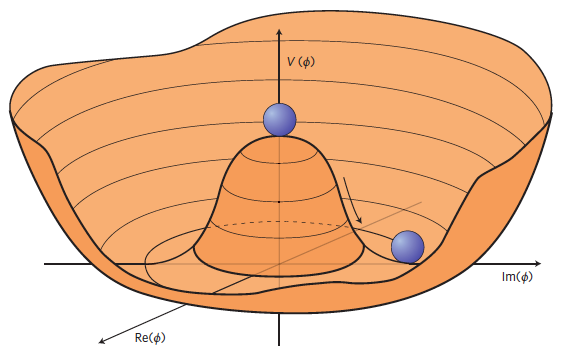
\includegraphics[scale=0.65]{figures/higgspotential}
\caption{The Higgs potential (from http://cds.cern.ch/record/1638469/plots) }
\label{Fig:higgspot}
\end{center}
\end{figure}

\indent In QED, the five gauge bosons are ${W^{i}_{\mu}, i = 1,2,3}$ and ${B_{\mu}}$. These bosons couple to a complex scalar Higgs doublet, ${\Phi \equiv \binom{\phi^{+}}{\phi^{0}}}$. This doublet has a scalar potential.
\begin{equation}
V(\Phi) = \mu^{2}|\Phi^{\dagger}\Phi| + \lambda(|\Phi^{\dagger}\Phi|)^{2}
\end{equation}
Where ${\mu^{2} < 0}$. This gives the Mexican hat shaped potential seen in figure ~\ref{Fig:higgspot}, with a minimum energy at 
\begin{equation}
\langle \phi \rangle = \sqrt{-\frac{\mu^{2}}{2\lambda}}\equiv \frac{\nu}{\sqrt{2}}
\end{equation}
called the vacuum expectation value (VEV) of ${\phi}$. The choice of the direction of fluctuation is arbitrary but can be chosen such that


 
\begin{equation}
\phi_{0} = \frac{1}{\sqrt{2}} \binom{0}{\nu}
\end{equation}
After the direction is chosen and the only remaining piece is the scalar field h(x), giving 
\begin{equation}
\phi(x) = \phi_{0} + h(x)
\end{equation}
The doublet can now be described by 
\begin{equation}
\Phi = \frac{1}{sqrt{2}} \binom{0}{v+h(x)}
\end{equation}
The Higgs field couples to the gauge bosons as 
\begin{equation}
(\frac{g}{2}\overrightarrow{\tau}\cdot \overrightarrow{W} + \frac{g'}{2}B)\phi_{0}
\end{equation}
Where ${\overrightarrow{\tau}}$ are the Pauli matrices, ${\overrightarrow{W}}$ are ${W_{1,2,3}}$ and g, g' are the coupling constants. The result of the coupling is the acquisition of mass by three eigenstates of the bosons, 
\begin{equation}
\begin{split}
W^{\pm} = \frac{1}{\sqrt{2}}(W^{1}_{\mu} \mp iW^{2}_{\mu})\\
Z^{\mu} = \frac{-g'B_{\mu} + gW^{3}_{\mu}}{\sqrt{g^{2} + g'^{2}}}\\
A^{\mu} = \frac{gB_{\mu} + g'W^{3}_{\mu}}{\sqrt{g^{2} + g'^{2}}}
\end{split}
\end{equation}
These four eigenstates are the bosons we observe in the standard model. With Masses
\begin{equation}
\begin{split}
M^{2}_{W} = \frac{1}{4}g^{2}\nu^{2} \\
M^{2}_{Z} = \frac{1}{4}(g^{2} + g'^{2})\nu^{2} \\
M_{A} = 0
\end{split}
\end{equation}
Through the mixing that occurs in the spontaneous electroweak symmetry breaking gives mass to the standard model Gauge Bosons while leaving the photon massless. However, for this to occur, an additional scalar field, the Higgs Field, is required.\linebreak
\indent The Higgs Boson is an excitation in the scalar Higgs field predicted in 1964. The decay mechanism of this massive boson was predicted by Peter Higgs, allowing for the decay products to be measured. Giving a way to prove the existence of the scalar Higgs field. In 2012, a Higgs like scalar boson was discovered at the LHC by the ATLAS and CMS experiments with a mass of 125GeV/c\textsuperscript{2} (ref XXX https://arxiv.org/abs/1207.7214). Since the discovery, many measurements have been made of this Higgs Boson to compare it to the standard model Higgs Boson. So far, the Higgs Boson has held up to these tests. The Higgs Boson has spin-parity J\textsuperscript{P} = 0\textsuperscript{+} 
(ref XXX %https://www.sciencedirect.com/science/article/pii/S0370269313006527?via%3Dihub)
, decays to bb (https://www.sciencedirect.com/science/article/pii/S0370269318307056), ${\gamma\gamma, \tau\tau}$,(ref XXX https://arxiv.org/abs/1811.08856) WW and ZZ have been measured with appropriate signal strengths, and no significant deviations have been observed in any Run 2 analyses. However, there are still many parameters of the Higgs Boson that still need measured. One of which is the triple Higgs coupling.
%Do I want to include more about the higgs discovery. 

%%\clearpage
%%-------------------------------------------------------------------------------
%
%
%%%-------------------------------------------------------------------------------
%\input{ATLASdetector}
%%\clearpage
%%-------------------------------------------------------------------------------
%
%%%-------------------------------------------------------------------------------
%\input{TriggerData}
%%\clearpage
%%-------------------------------------------------------------------------------
%
%
%%%-------------------------------------------------------------------------------
%\input{Simulation}
%%\clearpage
%%-------------------------------------------------------------------------------
%
%
%%%-------------------------------------------------------------------------------
%\input{Reconstruction}
%%\clearpage
%%-------------------------------------------------------------------------------
%
%
%%-------------------------------------------------------------------------------
%\input{SignalRegions}
%%\clearpage
%%%-------------------------------------------------------------------------------
%
%
%%%-------------------------------------------------------------------------------
%\input{Background}
%%\clearpage
%%-------------------------------------------------------------------------------
%
%
%%%-------------------------------------------------------------------------------
%\input{Systematics}
%%\clearpage
%%-------------------------------------------------------------------------------
%
%
%%%-------------------------------------------------------------------------------
%\input{Results}
%\clearpage
%%-------------------------------------------------------------------------------
%
%%
%%% All figures and tables should appear before the summary and conclusion.
%%% The package placeins provides the macro \FloatBarrier to achieve this.
%%% \FloatBarrier
%%
%%
%%-------------------------------------------------------------------------------
%\input{Conclusions}
%%\clearpage
%%%-------------------------------------------------------------------------------
%%
%%-------------------------------------------------------------------------------
%%%-------------------------------------------------------------------------------
%%
%
%
%%The \texttt{atlaslatex} package contains the acknowledgements that were valid 
%%at the time of the release you are using.
%%These can be found in the \texttt{acknowledgements} subdirectory.
%%When your ATLAS paper or PUB/CONF note is ready to be published,
%%download the latest set of acknowledgements from:\\
%%\url{https://twiki.cern.ch/twiki/bin/view/AtlasProtected/PubComAcknowledgements}
%
%%The supporting notes for the analysis should also contain a list of contributors.
%%This information should usually be included in \texttt{mydocument-metadata.tex}.
%%The list should be printed either here or before the table of contents.
%
%
%%-------------------------------------------------------------------------------
%%\clearpage
%%\appendix
%%\part*{Appendix}
%%\addcontentsline{toc}{part}{Appendix}
%%%-------------------------------------------------------------------------------
%%
%%In a paper, an appendix is used for technical details that would otherwise disturb the flow of the paper.
%%Such an appendix should be printed before the Bibliography.
%
%
%-------------------------------------------------------------------------------
% If you use biblatex and either biber or bibtex to process the bibliography
% just say \printbibliography here

\printbibliography
%\printbibliography[title={REFERENCES CITED},heading=bibintoc]


%\bibliographystyle{atlasBibStyleWithTitle}
%\bibliography{CONF}
% If you want to use the traditional BibTeX you need to use the syntax below.
%\bibliographystyle{bibtex/bst/atlasBibStyleWoTitle}
%\bibliography{atlas-document,bibtex/bib/ATLAS}
%-------------------------------------------------------------------------------

%-------------------------------------------------------------------------------
% Print the list of contributors to the analysis
% The argument gives the fraction of the text width used for the names
%-------------------------------------------------------------------------------
%\clearpage
%\PrintAtlasContribute{0.30}

%%-------------------------------------------------------------------------------


%\clearpage


%\appendix
%\input{auxMaterial}
%\appendix
%%\part*{Auxiliary material}
%%\addcontentsline{toc}{part}{Auxiliary material}
%%-------------------------------------------------------------------------------

%In an ATLAS paper, auxiliary plots and tables that are supposed to be made public 
%should be collected in an appendix that has the title \enquote{Auxiliary material}.
%This appendix should be printed after the Bibliography.
%At the end of the paper approval procedure, this information can be split into a separate document
%-- see \texttt{atlas-auxmat.tex}.
%
%In an ATLAS note, use the appendices to include all the technical details of your work
%that are relevant for the ATLAS Collaboration only (e.g.\ dataset details, software release used).
%This information should be printed after the Bibliography.

\end{document}
